%%
% Please see https://bitbucket.org/rivanvx/beamer/wiki/Home for obtaining beamer.
%%
\documentclass{beamer}
\usefonttheme{professionalfonts}
\usepackage{tikz}
\usetikzlibrary{trees}
\tikzset{
  invisible/.style={opacity=0},
  visible on/.style={alt={#1{}{invisible}}},
  alt/.code args={<#1>#2#3}{%
    \alt<#1>{\pgfkeysalso{#2}}{\pgfkeysalso{#3}} % \pgfkeysalso doesn't change the path
  },
  properties/.style={green, ultra thick},
}

\usepackage{amssymb,amsmath}

%\usepackage{refcheck}

\usepackage{graphicx}
\usepackage{amssymb}
\usepackage{mathrsfs}
\usepackage{amsmath}
\usepackage{latexsym}
\usepackage{amssymb}
\usepackage{enumerate}
\usepackage{color}
%\usepackage{ dsfont }
\usepackage{float}
\usepackage{physics}

%new math symbols taking no arguments
\newcommand\0{\mathbf{0}}
\newcommand\CC{\mathbb{C}}
\newcommand\FF{\mathbb{F}}
\newcommand\NN{\mathbb{N}}
\newcommand\QQ{\mathbb{Q}}
\newcommand\RR{\mathbb{R}}
\newcommand\ZZ{\mathbb{Z}}
\newcommand\bb{\mathbf{b}}
\newcommand\kk{\Bbbk}
\newcommand\mm{\mathfrak{m}}
\newcommand\pp{\mathfrak{p}}
\newcommand\xx{\mathbf{x}}
\newcommand\yy{\mathbf{y}}
\newcommand\GL{\mathit{GL}}
\newcommand\into{\hookrightarrow}
\newcommand\nsub{\trianglelefteq}
\newcommand\onto{\twoheadrightarrow}
\newcommand\minus{\smallsetminus}
\newcommand\goesto{\rightsquigarrow}
\newcommand\nsubneq{\vartriangleleft}

%redefined math symbols taking no arguments
\newcommand\<{\langle}
\renewcommand\>{\rangle}
\renewcommand\iff{\Leftrightarrow}
\renewcommand\phi{\varphi}
\renewcommand\implies{\Rightarrow}

%new math symbols taking arguments
\newcommand\ol[1]{{\overline{#1}}}

%redefined math symbols taking arguments
\renewcommand\mod[1]{\ (\mathrm{mod}\ #1)}

%roman font math operators
\DeclareMathOperator\aut{Aut}

%for easy 2 x 2 matrices
\newcommand\twobytwo[1]{\left[\begin{array}{@{}cc@{}}#1\end{array}\right]}

%for easy column vectors of size 2
\newcommand\tworow[1]{\left[\begin{array}{@{}c@{}}#1\end{array}\right]}

%\newtheorem{theorem}{Theorem}[section]
%\newtheorem{corollary}{Corollary}[theorem]
\newtheorem{proposition}{Proposition}[theorem]
\newtheorem{algorithm}{Algorithm}[theorem]
%\newtheorem{lemma}[theorem]{Lemma}
%\newtheorem{exercise}[theorem]{Exercise}
%\newtheorem{definition}[theorem]{Definition}

\title{Some Results in Quantum Learning Theory}
\author[Sbahi] % (optional, for multiple authors)
{Faris Sbahi}
\date{3/5/19}
\subject{Physics}

\begin{document}
\maketitle

\AtBeginSection[]
{
  \begin{frame}<beamer>
    \tableofcontents[currentsection]
  \end{frame}
}

\section{Dequantization}

\subsection{Quantum Machine Learning: "Read the Fine Print"}

\begin{frame}
\frametitle{Fine Print}
\begin{itemize}
\item In general, quantum machine learning algorithms convert quantum input states to the desired quantum output states. 
\item In practice, data is initially stored classically and the algorithm's output must be accessed classically as well.
\item Highlight: A practical way to make comparisons between classical and quantum algorithms is to analyze classical algorithms under $\ell^2$ sampling conditions
\item Tang: linear algebra problems in low-dimensional spaces (say constant or polylogarithmic) likely can be solved "efficiently" under these conditions
\item Many of the initial practical applications of quantum machine learning were to problems of this type (e.g. Quantum Recommendation Systems - Kerendis, Prakash, 2016)
\end{itemize}
\end{frame}

%\begin{frame}
%    \frametitle{Machine Learning}
%    \framesubtitle{Introduction}
%    \begin{itemize}
%    \item Machine learning is a broad term for algorithms which are capable of finding patterns in data.
%    \item Fundamental goal: capture these patterns in a "model" that \textit{generalizes} to unseen data.
%    \item These algorithms have two components:
%    \begin{enumerate}
 %   \item A learning element. Updates the model depending on its performance on the considered dataset.
 %   \item A performance element. Provides the measure of performance.
%    \end{enumerate}
%	\item Bottom line: "machine learning" is a somewhat hollow term. Many ML algorithms are in fact familiar linear algebraic techniques.
%    \end{itemize}
 %   \end{frame}

% Goal is simply to show why these linear algebraic techniques can be regarded as machine learning algorithms
  %\begin{frame}
%  	\frametitle{PCA}
%    \framesubtitle{Motivation: Singular value transformation}
%    \begin{itemize}
%    \item "Training" dataset $\mathcal{T}$ consists of the accessible samples of data. $\mathcal{T}$ is drawn from a subset of $\Omega \subset \RR^d$ where each component represents a "feature". 
 %   \item Samples from $\Omega$ are assumed to be drawn according to some distribution $\mathcal{D}$. 
 %   \pause
 %   \item Example: data is collected on the heights and lengths of cherry blossom petals. 
 %   \begin{figure}
 %  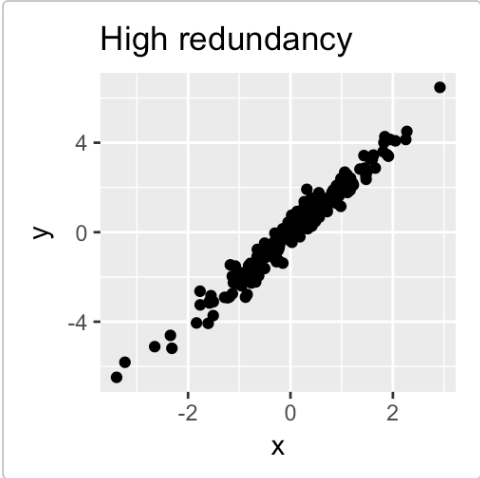
\includegraphics[width= 0.3\linewidth]{pca_high_redundancy.png}
 %  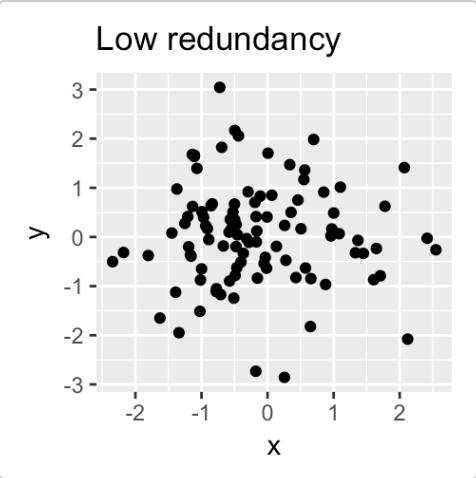
\includegraphics[width= 0.3\linewidth]{pca_low_redundancy}	
%\end{figure}
%\item How and why may it make sense to reduce the dimensionality of the feature space?
%\end{itemize}
%\end{frame}
%
%\begin{frame}
%\frametitle{Moore-Penrose Pseudoinverse}
 %   \framesubtitle{Motivation: Singular value transformation}
 %   \begin{itemize}
 %   \item Let $A \in \RR^{m \times n}$ and $b \in \RR^m$ unit vector. In machine learning, $A$ is the matrix with rows given by the samples of $\mathcal{T}$. 
    % We assume the distribution $\mathcal{D}$ now extends to $\Omega \times Y$, $Y \subset \RR$.
 %   \item We wish to find the $x_{LS}$ which satisfies $x_{LS} = \arg\min_{x} \| Ax - b \|_2$
 %   \item Notation: $x_{LS} = A^+ b$
 %   \pause
 %   \item Common strategy uses SVD: write $A = UDV^\dag$ and then $A^+ = VD^+U^\dag$ where $D^+$ simply inverts the non-zero diagonal entries.
 %   \end{itemize}
%	\begin{figure}
 %  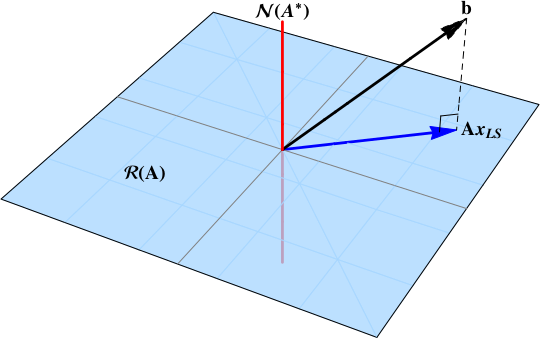
\includegraphics[width= 0.5\linewidth]{least-squares.png}	
%\end{figure}
%\end{frame}
%
%\section{Quantum Machine Learning}
%
%\begin{frame}
%\frametitle{Moore-Penrose Pseuodinverse (Quantum)}
%\framesubtitle{Harrow, Hassidim, Lloyd (orig.) Wiebe, Braun} 
%\begin{itemize}
    %\item HHL algorithm: application of phase estimation and Hamiltonian simulation to solve linear system.
%    \item We can compute $A^+ \ket{b} = \ket{x_{LS}}$ in $\tilde{O}(log(N)(s^3\kappa^6)/ \epsilon)$ time (query complexity)
 %   \item Uses a quantum algorithm based on phase estimation and Hamiltonian simulation
 %   \item Assumption: $A$ is sparse with low condition number $\kappa$. Hamiltonian ($\hat{H}$) simulation is efficient when $\hat{H}$ is sparse. No low-rank assumptions are necessary.
  %  \item "Key" assumption: the quantum state $\ket{b}$ can be prepared efficiently.	
 %   \item What happens if we assume low rank?
%\end{itemize}
%\end{frame}

\subsection{Classical $\ell^2$ sampling}

\begin{frame}
\frametitle{In search of a "fair" comparison}	

\begin{itemize}
\item How can we compare the speed of quantum algorithms with quantum input and quantum output to classical algorithms with classical input and classical output? 
\item Quantum machine learning algorithms can be exponentially faster than the best standard classical algorithms for similar tasks, but quantum algorithms get help through input state preparation. 
\item Want a practical classical model that helps its algorithms offer similar guarantees to quantum algorithms, while still ensuring that they can be run in nearly all circumstances one would run the quantum algorithm. 
\pause
\item Solution (Tang): compare quantum algorithms with quantum state preparation to classical algorithms with sample and query access to input.	
\end{itemize}
\end{frame}

% how to compare? query complexity
% what kind of data structure allows for l-s sampling

\begin{frame}
\frametitle{Classical $\ell^2$ Sampling Model}
\begin{definition}
We have "query access" to $x \in \CC^n$ if, given $i \in [n]$, we can efficiently compute $x_i$. We say that $x \in \mathcal{Q}$.
\end{definition}
\begin{definition} We have sample \textbf{and} query access to $x \in \CC^n$ if 

\begin{enumerate}
\item We have query access to $x$ i.e. $x\in \mathcal{Q}$ ($\implies$ $\mathcal{SQ} \subset \mathcal{Q}$)
\item can produce independent random samples $i \in [n]$ where we sample $i$ with probability $|x_i|^2/\|x\|^2∣$ and can query for $\|x\|$.
\end{enumerate}
We say that $x \in \mathcal{SQ}$. 
\end{definition}
\begin{definition} For $A \in \CC^{m\times n}$, $A \in \mathcal{SQ}$ (abuse) if

\begin{enumerate}
\item $A_i \in \mathcal{SQ}$ where $A_i$ is the $i$th row of $A$
\item $\tilde{A} \in \mathcal{SQ}$ for $\tilde{A}$ the vector of row norms (so $\tilde{A}_i = \|A_i\|$).	
\end{enumerate}
 
\end{definition}
\end{frame}

\begin{frame}
\frametitle{Example Data Structure}

Say we have the vector $\vec{x} = (2, 0, 1, 3)$ and $\vec{x} \in \mathcal{SQ}$. Consider the following binary tree data structure.

\begin{tikzpicture}[level distance=1.5cm,
  level 1/.style={sibling distance=5.5cm},
  level 2/.style={sibling distance=3cm}, 
  level 3/.style={sibling distance=3cm}]
  \node (1){$\| x \|^2 = 14$}
    child {node {$x_1^2 + x_2^2 = 4$}
      child {node {$x_1^2 = 4$}
      	child {node {$\text{sgn}(x_1) = +1$}}
      	edge from parent node [left] {\tiny $1$}
      }
      child {node {$x_2^2 = 0$} 
      	child {node {$\text{sgn}(x_2) = +1$}}
      	edge from parent node [right] {\tiny $0$}
      }
      edge from parent node [left] {\tiny $4/14$}
    }
    child {node(2) {$x_3^2 + x_4^2 = 10$}
    	child {node {$x_3^2 = 1$}
    		child {node {$\text{sgn}(x_3) = +1$}}
    		edge from parent node [left] {\tiny $1/10$}
    	}
      child {node(3) {$x_4^2 = 9$} 
      		child {node {$\text{sgn}(x_4) = +1$}}
      		edge from parent node [right] {\tiny $9/10$}
      } 
      edge from parent node [right] {\tiny $10/14$}
    };
    
    \only<2, 3>{\path(1)[->] edge[properties] (2);}
    \only<3>{\path(2)[->] edge[properties] (3);}
\end{tikzpicture}
\end{frame}

\begin{frame}
\frametitle{Dequantization Toolbox}
\framesubtitle{Method 1: Inner product estimation (Tang, 2018)}
\begin{itemize}
	\item For $x, y \in \CC^n$, if we are given that $x \in \mathcal{SQ}$ and $y \in \mathcal{Q}$, then we can estimate $\< x, y\>$ with probability $\geq 1 - \delta$ and error $\epsilon \|x\|\|y\|$ 
	\pause
	\item Quantum analog: SWAP test
\end{itemize}
%\begin{figure}
%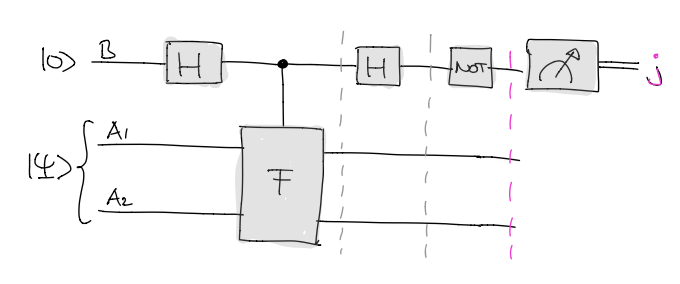
\includegraphics[width= 0.5\linewidth]{swap_test.png}	
%\end{figure}
\end{frame}

\begin{frame}
\frametitle{Dequantization Toolbox}
\framesubtitle{Method 1: Inner product estimation (Tang, 2018)}
\begin{fact} For $\{X_{i,j}\}$ i.i.d random variables with mean $\mu$ and variance $\sigma^2$, let 

$$Y := \underset{j \in [\log 1/\delta]}{\operatorname{median}}\;\underset{i \in [1/\epsilon^2]}{\operatorname{mean}}\;X_{i,j}$$

Then $\vert Y - \mu\vert \leq \epsilon\sigma$ with probability $\geq 1-\delta$, using only $O(\frac{1}{\epsilon^2}\log\frac{1}{\delta})$ samples.
\end{fact}

\begin{itemize}
	\item In words: We may create a mean estimator from $1/\epsilon^2$ samples of $X$. We compute the median of $\log 1/\delta$ such estimators
	\pause
	\item Catoni (2012) shows that Chebyshev's inequality is the best guarantee one can provide when considering pure empirical mean estimators for an unknown distribution (and finite $\mu, \sigma$)
	\item "Median of means" provides an exponential improvement in probability of success ($1 - \delta$) guarantee
\end{itemize}
%\begin{proof} (sketch) The proof follows from two facts:
%\begin{itemize}
%\item first, the median of $n$ random variables $C_1,\ldots,C_n$ is at least some constant $\lambda$ precisely when at least half of the $C_i$ are at least $\lambda$; 
%\item second, Chebyshev's inequality (applied to the mean).
%\end{itemize}
%\end{proof}
\end{frame}

\begin{frame}
\frametitle{Dequantization Toolbox}
\framesubtitle{Method 1: Inner product estimation (Tang, 2018)}
\begin{corollary} For $x,y \in\CC^n$, given $x \in \mathcal{SQ}$ and $y \in \mathcal{Q}$, we can estimate $\langle x,y\rangle$ to $\epsilon\|x\|\|y\|$ error with probability $\geq 1-\delta$ with query complexity $O(\frac{1}{\epsilon^2}\log\frac{1}{\delta})$
\end{corollary}
\pause
\begin{proof}Sample an \textbf{index} $s$ from $x$. Then, define $Z := x_s y_s\frac{\|y\|^2}{|y_s|^2}$. Apply the Fact with $X_{i,j}$ being independent samples $Z$.
\end{proof}	
\end{frame}

\begin{frame}
\frametitle{Dequantization Toolbox}
\framesubtitle{Method 2: Thin Matrix-Vector (Tang, 2018)}
\begin{itemize}
	\item For $V \in \CC^{n\times k}, w \in \CC^k$, given $V^\dagger \in \mathcal{SQ}$ (\textit{column}-wise sampling of $V$) and $w \in \mathcal{Q}$, we can simulate $Vw \in \mathcal{SQ}$ with $\text{poly}(k)$ queries
	\item In words: if we can least-square sample the columns of matrix $V$ and query the entries of vector $w$, then
\begin{enumerate}
\item  We can query entries of their multiplication ($Vw$) 
\item We can least-square sample from a distribution that emulates their multiplication	
\end{enumerate}

\item Hence, as long as $k \ll n$, we can perform  each using a number of steps polynomial in the number of columns of $V$. 

\end{itemize}
\end{frame}

\begin{frame}
\frametitle{Dequantization Toolbox}
\framesubtitle{Method 2: Thin Matrix-Vector (Tang, 2018)}
\begin{definition}
Rejection sampling
\end{definition}
\begin{algorithm}
Input: Samples from distribution $P$

Output: Samples from distribution $Q$
\begin{itemize}
\item Sample $s$ from $P$
\item Compute $r_s = \frac{1}{N}\frac{Q(s)}{P(s)}$, for fixed constant $N$
\item Output $s$ with probability $r_s$ and restart otherwise
\end{itemize}
\end{algorithm}

\begin{fact}
Fact. If $r_i \leq 1, \forall i$, then the above procedure is well-defined and outputs a sample from $Q$ in $N$ iterations in expectation.	
\end{fact}


\end{frame}

\begin{frame}
\frametitle{Dequantization Toolbox}
\framesubtitle{Method 2: Thin Matrix-Vector (Tang, 2018)}
\begin{proposition}
	 For $V \in \RR^{n\times k}$ and $w \in \RR^k$, given $V^\dag \in \mathcal{SQ}$ and $w \in \mathcal{Q}$, we can simulate $Vw \in \mathcal{SQ}$ with expected query complexity $\tilde{O}((\frac{1}{\epsilon^2}\log\frac{1}{\delta}))$

We can compute entries $(Vw)_i$ with $O(k)$ queries.

We can sample using rejection sampling:

\begin{itemize}
\item $P$ is the distribution formed by sampling from $V_{(\cdot, j)}$.
  
\item $Q$ is the target $Vw$.
\item Hence, compute $r_s$ to be a constant factor of $Q / P$
\end{itemize}

$$r_i = \frac{\|w^T V_{\cdot, i}\|^2}{\|w\|^2\|V_{\cdot, i}\|^2}$$
\end{proposition}
\end{frame}

\begin{frame}
\frametitle{Dequantization Toolbox}
\framesubtitle{Method 2: Thin Matrix-Vector (Tang, 2018)}
\begin{itemize}
\item Notice that we can compute these $r_i$'s (in fact, despite that we cannot compute probabilities from the target distribution), and that the rejection sampling guarantee is satisfied (via Cauchy-Schwarz).

\item Since the probability of success is $\|Vw\|^2/ \| w\|^2$, it suffices to estimate the probability of success of this rejection sampling process to estimate this norm.

\item Through a Chernoff bound, we see that the average of $O(\|w\|^2(\frac{1}{\epsilon^2}\log\frac{1}{\delta}))$ "coin flips" is in $[(1-\epsilon)\|Vw\|,(1+\epsilon)\|Vw\|]$ with probability $\geq 1-\delta$.
\end{itemize}
\end{frame}


\begin{frame}
\frametitle{Dequantization Toolbox}
\framesubtitle{Method 3: Low-Rank Approximation (Frieze, Kannan, Vempala, 1998)}
\begin{itemize}
\item For $A \in \CC^{m\times n}$, given $A \in \mathcal{SQ}$ and some threshold $k$, we can output a description of a low-rank approximation of $A$ with $\text{poly}(k)$ queries.
\item Specifically, we output two matrices $S,\hat{U}\in \mathcal{SQ}$ where $S \in \CC^{\ell \times n}$, $\hat{U} \in \CC^{\ell \times k}$ ($\ell = \text{poly}(k,\frac{1}{\epsilon}$)), and this implicitly describes the low-rank approximation to $A$, $D := A(S^\dagger\hat{U})(S^\dagger\hat{U})^\dag$ ($\implies$ rank $D \leq k$).

\item This matrix satisfies the following low-rank guarantee with probability $\geq 1-\delta$: for $\sigma := \sqrt{2/k}\|A\|_F$, and $A_{\sigma} := \sum_{\sigma_i \geq \sigma} \sigma_iu_iv_i^\dag$ (using SVD), 
$$\|A - D\|_F^2 \leq \|A - A_\sigma\|_F^2 + \epsilon^2\|A\|_F^2$$
\item Note the $\|A - A_\sigma\|_F^2$ term. This says that our guarantee is weak if $A$ has no large singular values. 
\item Quantum analog: phase estimation
\end{itemize}
\end{frame}

\begin{frame}
\frametitle{Dequantization Toolbox}

$$
\begin{bmatrix}
\\
\cdots A \cdots 
\\
\\	
\end{bmatrix}
\begin{bmatrix}
\\
S^\dag
\\
\\	
\end{bmatrix}
\begin{bmatrix}
\hat{U}
\end{bmatrix}
\begin{bmatrix}
\hat{U^\dag}
\end{bmatrix}
\begin{bmatrix}
\cdots S \cdots
\end{bmatrix}
$$
​		
\end{frame}


\begin{frame}
\frametitle{Polynomial (low-rank)} 	
\framesubtitle{Application (Lloyd, Tang, 2018)}

\begin{problem} For a low-rank matrix $A \in \RR^{m\times n}$ with SVD $\sum_i \sigma_i \ket{u_i} \bra{v_i}$
  and a vector $b \in \RR^n$, given $b, A \in \mathcal{SQ}$, (approximately) simulate $\sum_i (\sigma_i)^m \ket{u_i} \bra{v_i} b \in \mathcal{SQ}$ for any $m \in \ZZ$.
\end{problem}
\begin{problem}
Special case: Moore-Penrose Pseuodinverse	
\end{problem}
\pause
\begin{algorithm}   	
\begin{itemize}
\item Algorithm: see the thesis!

\end{itemize}
\end{algorithm}
\end{frame}

\subsection{Remarks}

\begin{frame}
\frametitle{Thoughts}	

\begin{itemize}
\item Claim (Tang): For machine learning problems, $\mathcal{SQ}$ assumptions are more reasonable than state preparation assumptions.
\item We discussed pseudo-inverse which inverts singular values, but in principle we could have applied any function to the singular values
\item Gilyen et. al (2018) show that many quantum machine learning algorithms indeed apply polynomial functions to singular values
\item Our discussion suggests that exponential quantum speedups are tightly related to problems where high-rank matrices play a crucial role (e.g. Hamiltonian simulation or QFT)
\end{itemize}
\end{frame}


% mention qram?


% bonus slides

\begin{frame}
\frametitle{Read the Fine Print}	
\begin{itemize}
\item This poses two problems if seek to use these algorithms: the "state preparation" and "readout" problems.
\item Even if we ignore the readout problem, can we at least find a state preparation routine that maintains a speedup for the discussed quantum algorithms? Open question!
\item See "Quantum Machine Learning Algorithms: Read the Fine Print" by Aaronson
\end{itemize}
\end{frame}

\begin{frame}
\frametitle{"Dequantization" (Tang)}
\begin{definition}
 Let $\mathcal{A}$ be a quantum algorithm with input $\ket{\phi_1},\ldots,\ket{\phi_C}$ and output either a state $\ket{\psi}$ or a value $\lambda$. We say we dequantize $\mathcal{A}$ if we describe a classical algorithm that, given $\phi_1,\ldots,\phi_C \in \mathcal{SQ}$, can evaluate queries to $\psi \in \mathcal{SQ}$ or output $\lambda$, with similar guarantees to $\mathcal{A}$ and query complexity $\text{poly}(C)$.	
\end{definition}
\end{frame}

\section{Quantum Feature Maps}

\begin{frame}
\frametitle{Kernel Maps}
\begin{itemize}
\item SVM: construct a separating hyperplane such that the distance to the nearest training observation (minimum margin) is maximized
\item "kernel trick": implicitly maps the data to a higher dimensional space so that it is separable or approximately separable (implicit by Mercer's Theorem) 
\item Seek a linear function $f(x) = \vec{w} \cdot \vec{x}$ where $\vec{w}$ is a weight vector s.t. $y_if(x_i) > 0$ for all (or many) $i$
\item Input state preparation solution?
\end{itemize}

\begin{figure}[H]
\centering
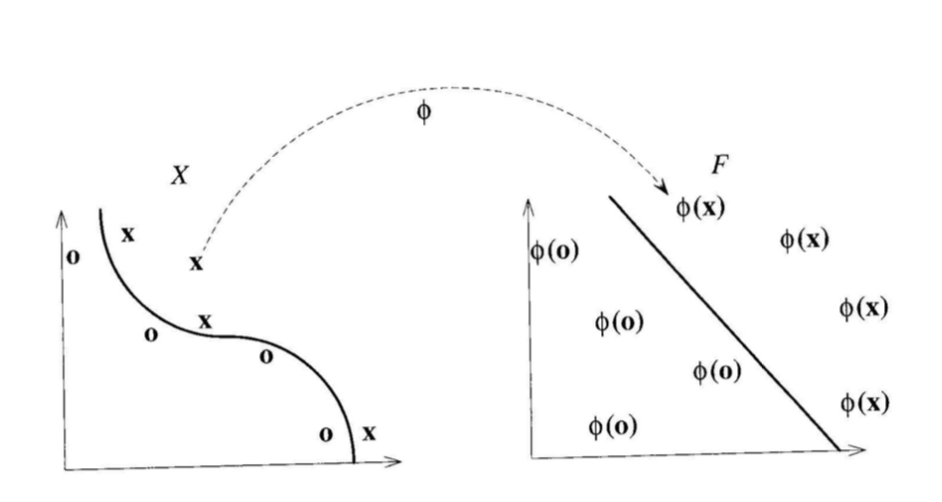
\includegraphics[width= 0.7\linewidth]{images/kernel}
\caption{Nonlinear boundary created by kernel map. Data is mapped to a higher dimensional space where a linear boundary is created, and then this boundary is mapped back to the original space (creating the nonlinearity).}
\end{figure}

\end{frame}

\begin{frame}	

\frametitle{The Shifted Bent Map}

Consider the feature map defined in Havlicek et. al (Nature Physics).

First define,

\begin{align}
\label{eq:diagonal-feat}
U_{\Phi(x)} &= \exp\Big(i \sum_{S \subseteq [n]} \phi_S(x) \prod_{i \in S} Z_i \Big)	
\end{align}

with nonlinear coefficients $\phi_S(x) \in \RR$. Then, the feature map is given by 


\begin{align}
\label{feat-map:hav}
\mathcal{U}_{\Phi(x)} &= U_{\Phi(x)} H^{\otimes n} U_{\Phi(x)} H^{\otimes n}
\end{align}

\begin{figure}[H]
\centering
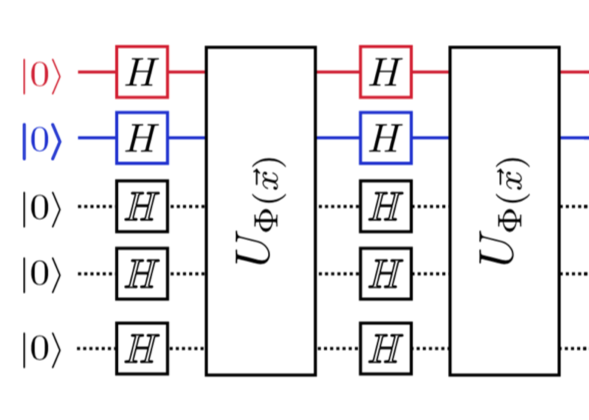
\includegraphics[width=0.5\textwidth]{images/feature_map_circuit}
\caption{Figure from \cite{havlicek2018supervised} of the feature map encoding circuit}
\end{figure}
\end{frame}

 
 \begin{frame}
\frametitle{Quantum Variational Classification}
\begin{enumerate}
\item Encode classical input data $\{\vec{x}_i \}$ as $\{\ket{\Phi(x_i)} \}$ ($\equiv \{\Phi(x_i)\ket{0} \}$) for some unitary feature map $\phi$

\item Apply a $\theta$-parameterized unitary $W(\theta)$ to the input state giving

\begin{align*}
W(\theta)\ket{\Phi(x_i)}
\end{align*}

\item Measure multiple shots of some observables $\{M\}$. The expectation value of these observables is utilized to output a real-valued prediction function $f : \{x_i\} \rightarrow \RR$.

\item Minimize a chosen cost function with is a function of $f(x_i)$. For example, the $\ell_2$ loss

\begin{align*}
\sum_i (y_i - f(x_i))^2	
\end{align*}

\item Evaluate the performance and update $\theta$ accordingly (e.g. using gradient descent). Return to step 2, or exit if done iterating.

\end{enumerate}
\end{frame}

\begin{frame}
\frametitle{Quantum Variational Classification: Continued}
A common choice of $W(\theta)$ (Figure \ref{fig:var}) is the following circuit: 

\begin{itemize}
\item Let $W(\theta)$ have $l$ layers i.e. $W(\theta) = W_1(\theta) \cdots W_l(\theta)$. 

\item Now, for each $W_i(\theta)$ we construct the following circuit: label the qubits $\{1, \cdots, n\}$ and consider the nearest-neighbor pairing $N = \{(1,2), (2, 3), \cdots, (n-1, n)\}$. Then, perform Control-Z on each pair in $N$. Next, write $\theta = (\theta_1, \cdots, \theta_n)$ where each $\theta_i$ is a vector specified by Euler angles. Hence, we can perform rotation $R(\theta_i)$ on the $i$th qubit.
\end{itemize}

\begin{figure}
\label{fig:var}
\centering
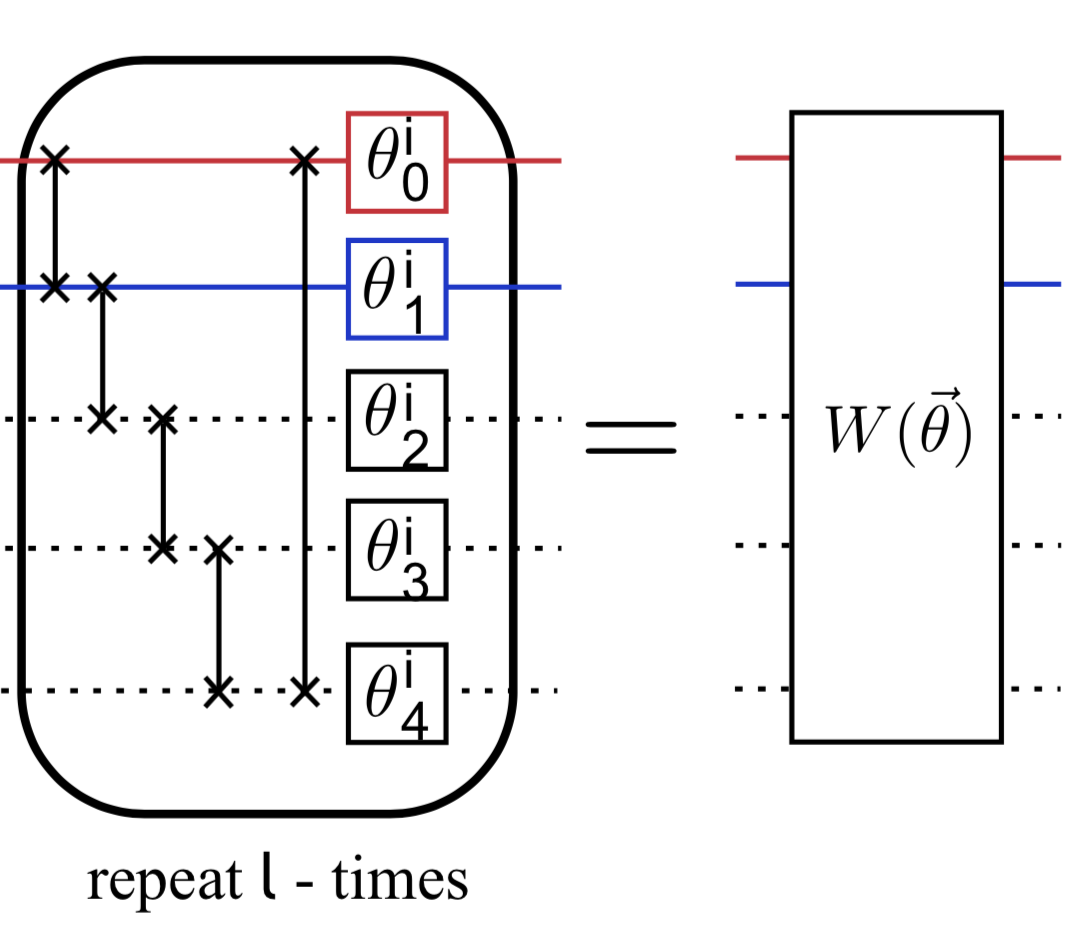
\includegraphics[width=0.5 \textwidth]{images/variational.png}	
\caption{Variational circuit diagrammed in \cite{havlicek2018supervised}}
\end{figure}
\end{frame}

%\section{Quantum Kernel Estimation}
%
%\section{Non-Trivial Feature Map with Entanglement}
%
%\section{Geometric Analysis of Candidate Feature Maps}
%
\section{Experimental Simulation of the Shifted Bent Feature Map}

\subsection{Separable Data}

\begin{frame}
Here, we demonstrate an experimental construction of the feature map defined in (\ref{feat-map:hav}) considering 2 qubits for data input. We use the Strawberry Fields package for simulation \cite{killoran2019strawberry}.

We generate data so that it can be perfectly separated. Choose coefficients

\begin{align*}
\phi_{i}(x) &= x_i, i \in \{1, 2\} \\
\phi_{\{1,2\}}(x) &= (\pi - x_1)(\pi - x_2) 
\end{align*}

and draw a fixed random element $V \in SU(4)$. Define $\Pi = Z_1Z_2$ to be parity on 2 qubits. Then, generate data by drawing (uniform) random $x \in (0, 2\pi]^2$ and labelling based on decision rule

\begin{align*}
f(x) = \bra{0} \mathcal{U}_{\Phi(x)}^\dag V^\dag \Pi V \mathcal{U}_{\Phi(x)}\ket{0}	 
\end{align*}

In particular, define a threshold $\Delta$ and if $|f(x)| \leq \Delta$ then draw another $x$. Otherwise, label by $sgn(f(x))$. We draw 40 such $x$ and arbitrary partition the dataset into training and test subsets of size 20 each.
\end{frame}

\begin{frame}
We then use the variational circuit described in the previous section to train our classifier. In particular, the variational circuit trains some $W(\theta)$ parameterized by $\theta$ and then constructs decision rule

\begin{align*}
\tilde{f}(x) &= \bra{0} \mathcal{U}_{\Phi(x)}^\dag W(\theta)^\dag \Pi W(\theta) \mathcal{U}_{\Phi(x)}\ket{0})
\end{align*}
 
and classifies by $sgn(\tilde{f}(x))$. In principle, then, because $W(\theta)$ can learn any $SU(4)$ gate for appropriately chosen $\theta$, we should be able to classify to near perfect accuracy. We use the "Nesterov momentum optimizer" to train $\theta$, an improvement of the usual stochastic gradient descent.
\end{frame}

\begin{frame}
Below, we plot the results of a few representative sample trials exploring various values of $\Delta$.

\begin{figure}[H]
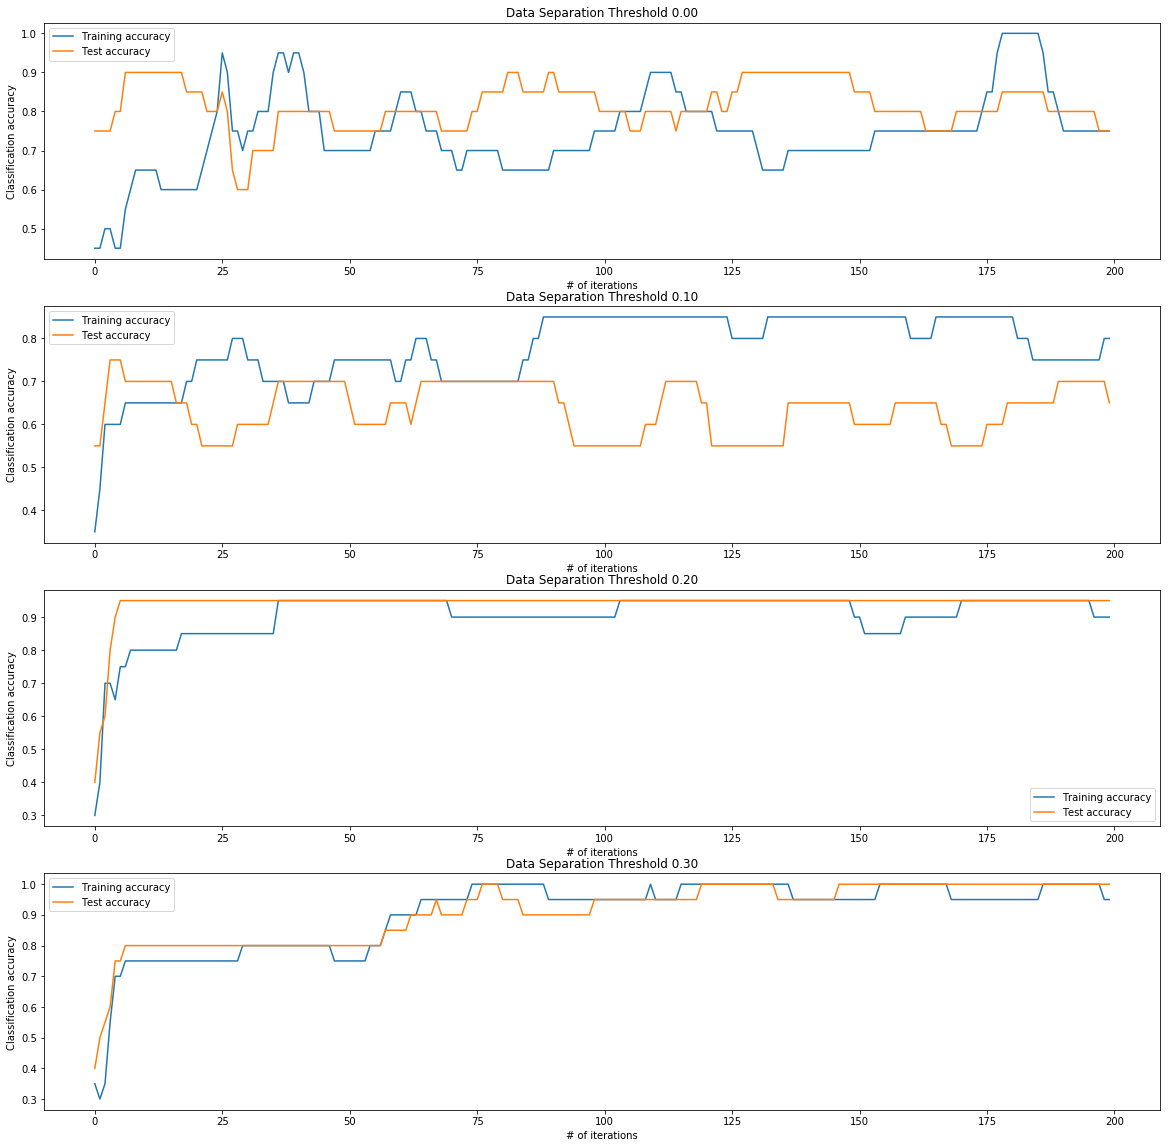
\includegraphics[width=0.5\textwidth]{images/data_sep}
\caption{A comparison of training and test convergence across varying data separations.}
\end{figure}
\end{frame}

\begin{frame}
Furthermore, can view the convergence of the dual $\ell^2$ loss view below.

\begin{figure}[H]
\centering
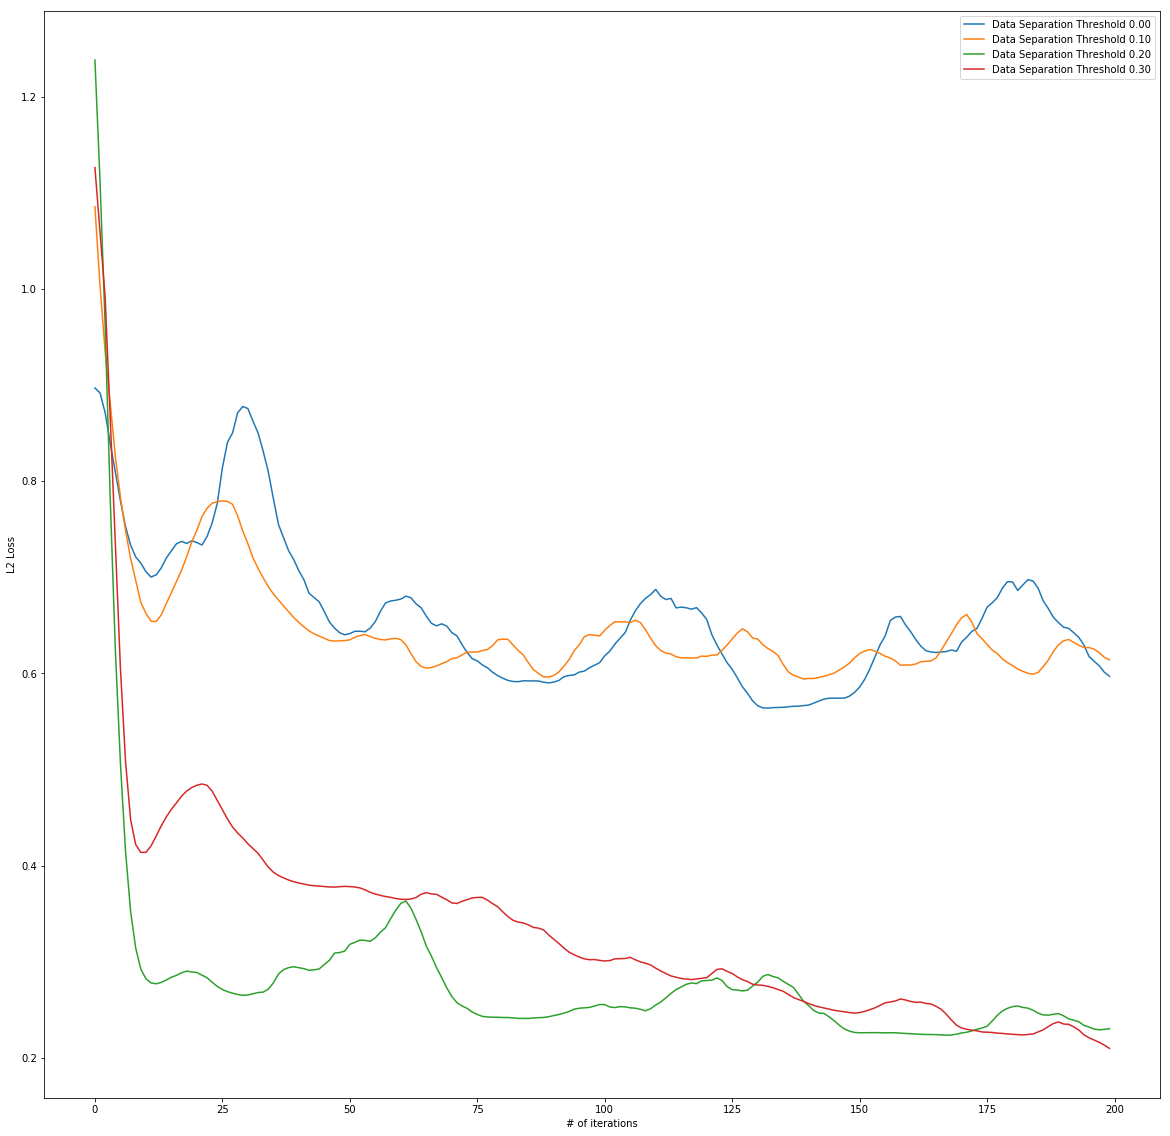
\includegraphics[width=0.5\textwidth]{images/l2_loss_conv}	
\caption{A similar comparison of $\ell^2$ loss convergence across varying data separations.}
\end{figure}
\end{frame}

\begin{frame}
Visually, generated data may look as below for some $V \in SU(4)$. We can visualize the decision boundary of the kernel by shading the regions in a color indicating the label which the classifier would output at each point.

\begin{figure}[H]
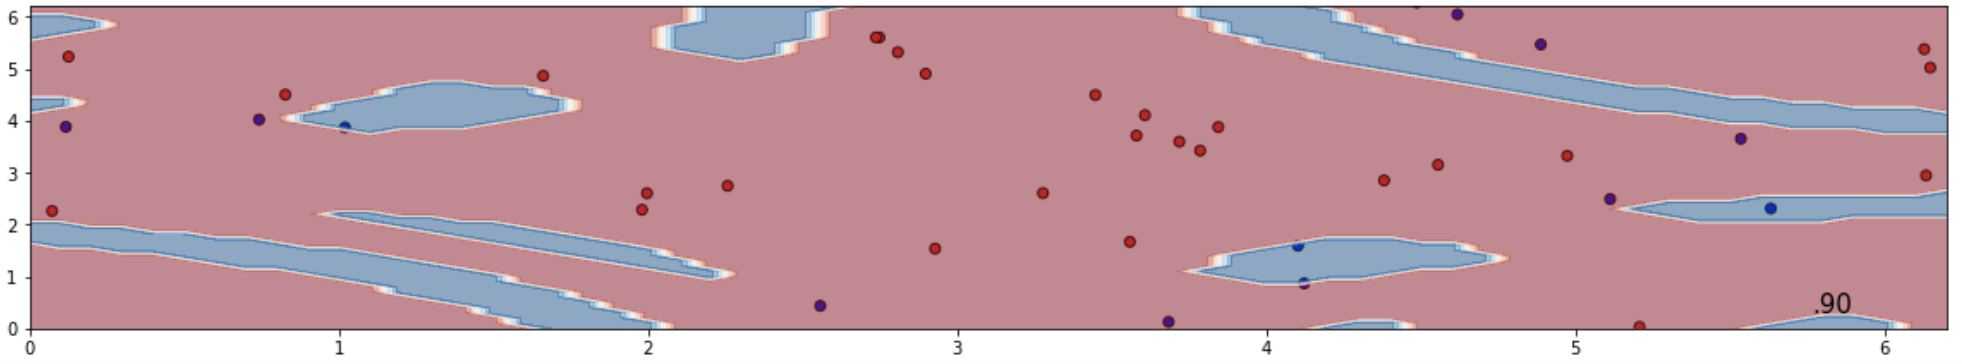
\includegraphics[width=\textwidth]{images/separable_data}
\caption{Sample output of the classifier. The colors of the regions indicate the label for which the classifier has learned for each point. The circles indicate data points in the generated set, colored by true label.}
\end{figure}
\end{frame}

\begin{frame}
We checked convergence for two separable datasets across the range of 1-5 layers, performing 20 trials per layer depth. Based on the preceding results, data separation of 0.3 was utilized in order to speed up convergence.

\begin{figure}[H]
\centering
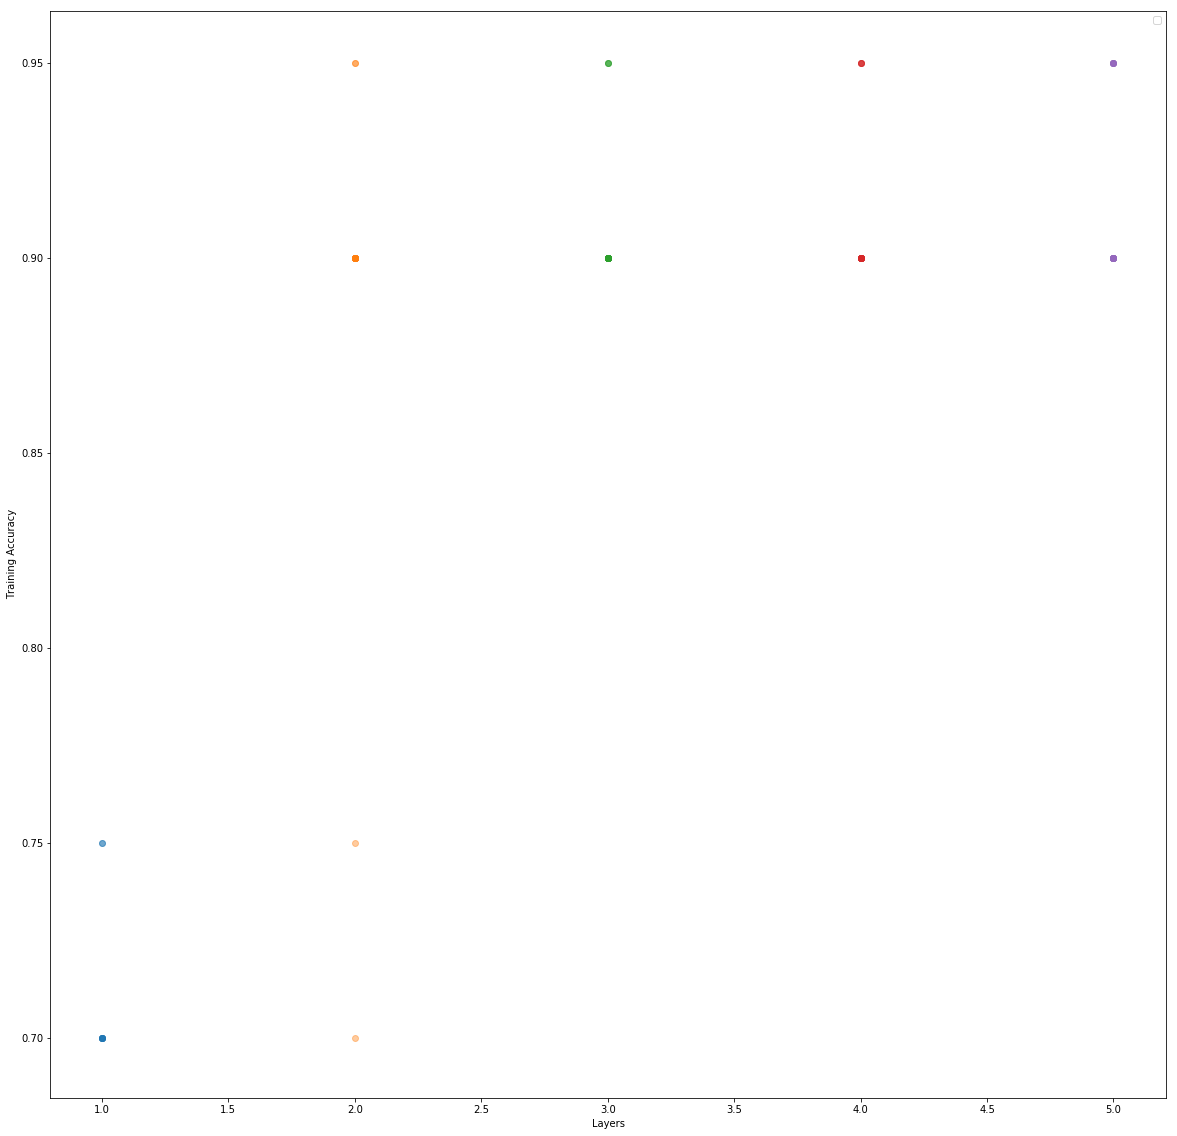
\includegraphics[width=0.5\textwidth]{images/train_accs_layer_sep.png}	
\caption{Training accuracy over repeated trials of 200 epochs varying over layer depth}
\end{figure}
\end{frame}

\begin{frame}
\begin{figure}[H]
\centering
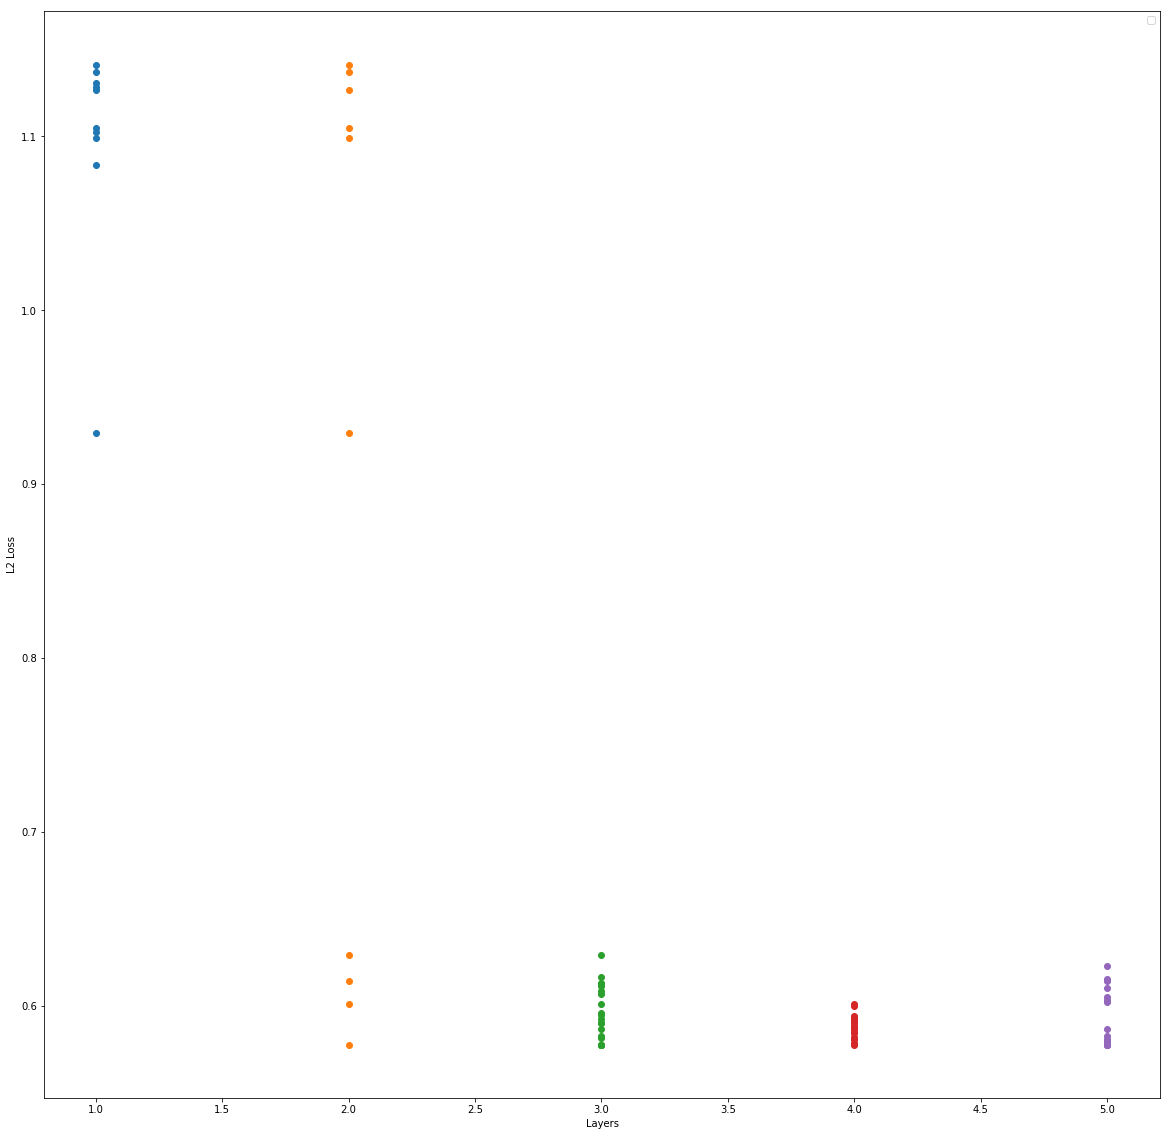
\includegraphics[width=0.7\textwidth]{images/costs_layer_sep.png}	
\caption{$\ell^2$ loss over repeated trials of 200 epochs varying over layer depth}
\end{figure}
\end{frame}

\subsection{Practical Data}

\begin{frame}
UCI ML Breast Cancer Dataset which contains 30 features and 569 samples. The labels correspond to whether a cell mass is malignant or benign. We apply PCA to reduce the dimensionality of the dataset to 2 and standardize to a centered Gaussian about $[0, \pi]$.

\begin{figure}[H]
\centering
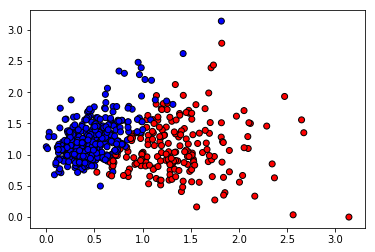
\includegraphics[width=0.7\textwidth]{images/breast_cancer_data}	
\end{figure}
\end{frame}

\begin{frame}
\begin{figure}[H]
\centering
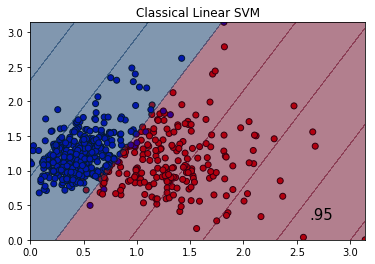
\includegraphics[width=0.7\textwidth]{images/breast_cancer_linear_svm}	
\end{figure}
\end{frame}

\begin{frame}
\begin{figure}[H]
\centering
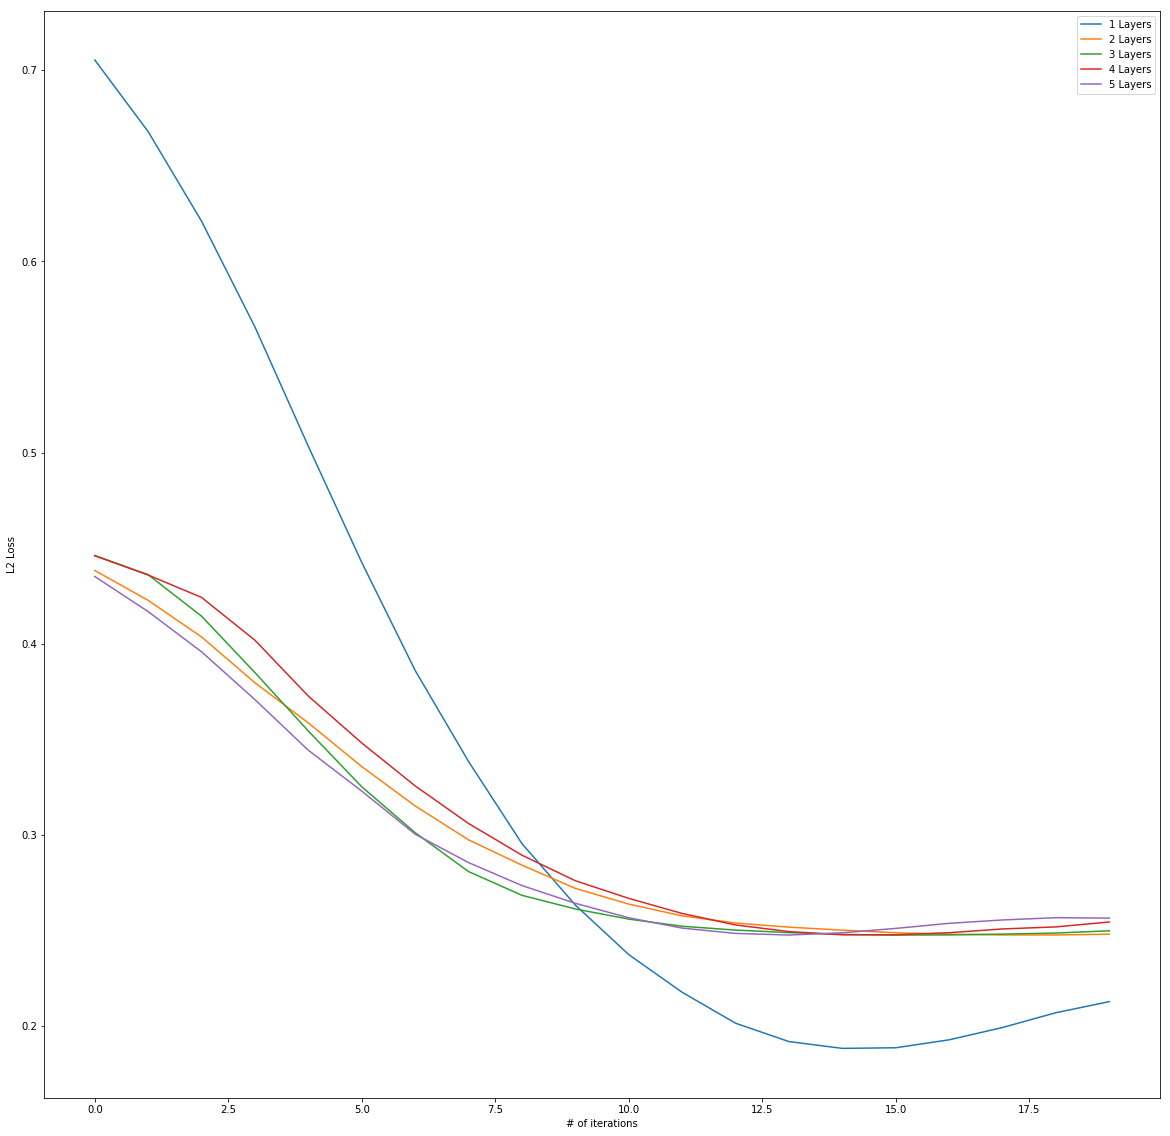
\includegraphics[width=0.7\textwidth]{images/breast_cancer_layers}	
\caption{The pattern in convergence in cost on the UCI Breast Cancer dataset is similar to the one for the separable dataset.}
\end{figure}
\end{frame}

\begin{frame}
\begin{figure}[H]
\centering
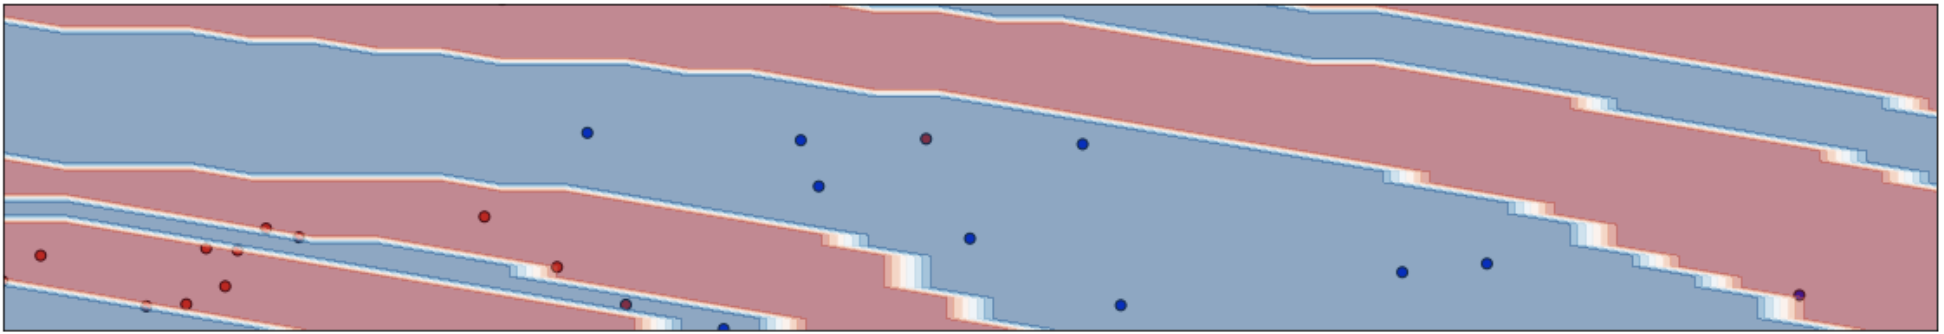
\includegraphics[width=0.7\textwidth]{images/practical_data_landscape}
\caption{Sample output of the classifier for the UCI Breast Cancer dataset}
\end{figure}
\end{frame}


% similar plot for costs

%
%\section{Density Matrix Exponentiation Algorithms}
%\url{https://www.nature.com/articles/nphys3029}
%
%\section{Review of Quantum Machine Learning}
%\url{https://www.nature.com/articles/nature23474}
%
%\section{Learnability of Quantum States}
%\begin{enumerate}
%\item \url{https://arxiv.org/abs/quant-ph/0608142}
%\item \url{https://arxiv.org/abs/1711.01053}
%\item \url{https://arxiv.org/abs/1801.05721}
%\end{enumerate}

\subsection{Moons Data}
\label{sec:moon}

\begin{frame}
\frametitle{Moons Data}	
We generate the data of this section by using the scikit-learn Python package and add random Gaussian noise to the $\{x_i\}$ for each trial.

\begin{figure}[H]
\centering
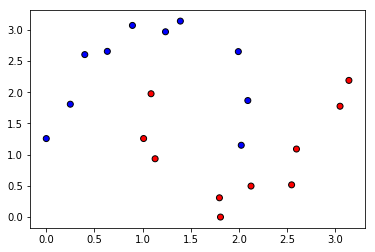
\includegraphics[width=0.7\textwidth]{images/moons_data}
\caption{Sample Moons data for some perturbation in Gaussian noise}
\end{figure}
\end{frame}

\begin{frame}
\begin{figure}[H]
\centering
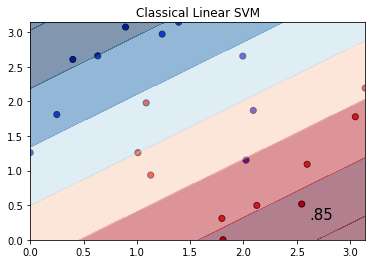
\includegraphics[width=0.7\textwidth]{images/moons_linear_svm}
\caption{Performance of SVM with a linear kernel on the Moons dataset}
\end{figure}

To see how the quantum feature map performs, we direct your attention to the next section.
\end{frame}

\section{Theoretical Extensions of the Shifted Bent Feature Map}

\subsection{A Connection Between State Tomography and Hyper-parameter Tuning}

\begin{frame}
We consider introducing a set of hyper-parameters which tunes the extent to which nonlinearity enters the phase of the $U_{\Phi(x)}$ (Equation \ref{eq:diagonal-feat}). We can revise the diagonal (in the $Z$ basis) unitary within the feature map:

\begin{align*}
U_{\Phi(x; \vec{\gamma})} &= \exp\Big(i \Big[\sum_{i} \phi_i(x) Z_i + \gamma_1 \sum_{i,j} \phi_{i,j}(x) Z_i Z_j + \cdots +  \\
&t\gamma_{d-1} \sum_{S \subseteq [d], |S| = d} \phi_S(x) \prod_{i \in S} Z_i \Big]\Big)	
\end{align*}

\end{frame}

\begin{frame}
Figure \ref{fig:breast_cancer_gammas} offers a representative view of how adjusting the single $\gamma$ hyper-parameter for the 2-qubit map adjusts the classification circuit to which the variational algorithm converges after 200 epochs when considering the UCI Breast Cancer dataset.
\end{frame}

\begin{frame}
\begin{figure}[H]
\label{fig:breast_cancer_gammas}
\centering
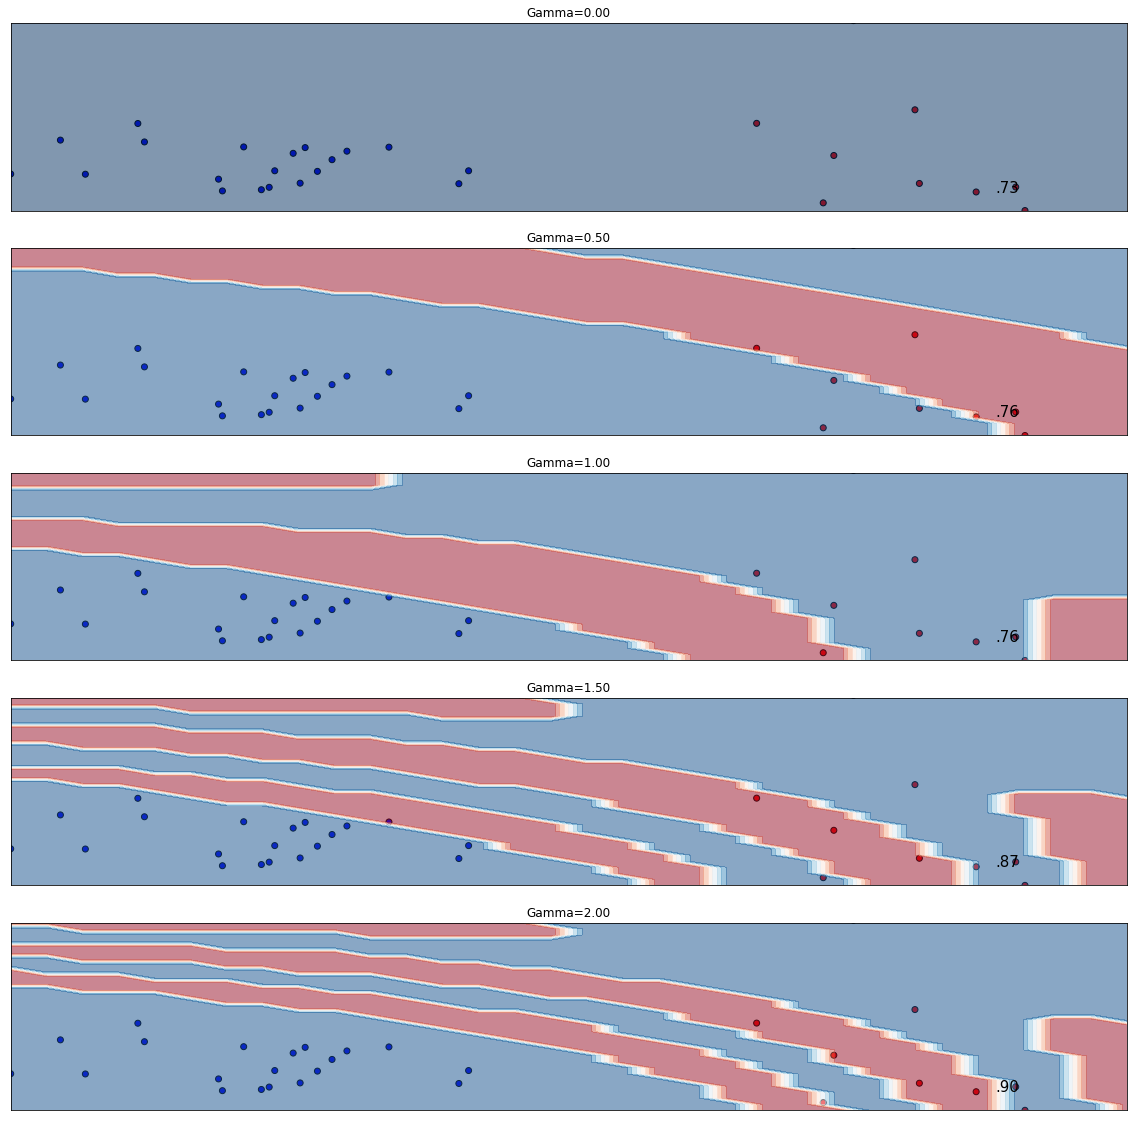
\includegraphics[width=0.7\textwidth]{images/breast_cancer_gammas}	
\caption{Performance of the variational classification circuit (for 200 epochs) on a random sample of the UCI Breast Cancer dataset for varying 2-point nonlinearity parameter $\gamma$.}
\end{figure}
\end{frame}

\begin{frame}
We contribute a novel method of thinking about tuning hyper-parameters for a quantum feature map and additionally demonstrate that the method works well in practice by returning to the "moons" binary classification problem of Section \ref{sec:moon}.

First, we make the straightforward observation that the goal of the variational classifier can be restated as solving a state identification problem:

Write that a data point $x$ is encoded as

\begin{align*}
\ket{\Phi(x; \vec{\gamma})} \equiv \mathcal{U}_{\Phi(x; \vec{\gamma})}\ket{0}
\end{align*}

Then, consider the density matrices

\begin{align*}
\rho_+ &= \frac{1}{N_+} \sum_{x_i : y_i = +1} \ket{\Phi(x_i; \vec{\gamma})}\bra{\Phi(x_i; \vec{\gamma})}	\\
\rho_- &= \frac{1}{N_-} \sum_{x_i : y_i = -1} \ket{\Phi(x_i; \vec{\gamma})}\bra{\Phi(x_i; \vec{\gamma})}	
\end{align*}

\end{frame}

\begin{frame}

Therefore, the goal of binary classification can be restated as finding the optimal pair of POVMs so as to maximize the probability of correctly distinguishing these two density matrices. The trace distance provides an achievable (by the Helstrom measurement) upper bound for solving this state identification problem. 

Hence, our method of hyperparameter tuning can be stated as follows: (1) compute the density matrices $\rho_+, \rho_-$ above for a set of candidate $\{ \vec{\gamma_i} \}$ (2) computing the trace distance $T(\rho_+, \rho_-)$ across the set of $\{ \vec{\gamma_i} \}$, and (3) choose the $\vec{\gamma_i}$ which maximizes trace distance. 

\end{frame}

\begin{frame}
For the dataset of Figure \ref{fig:breast_cancer_gammas}, we indeed see that trace distance increases with gamma within the range $[0.0, 2.0]$.
\end{frame}
\begin{frame}
\begin{figure}[H]
\centering
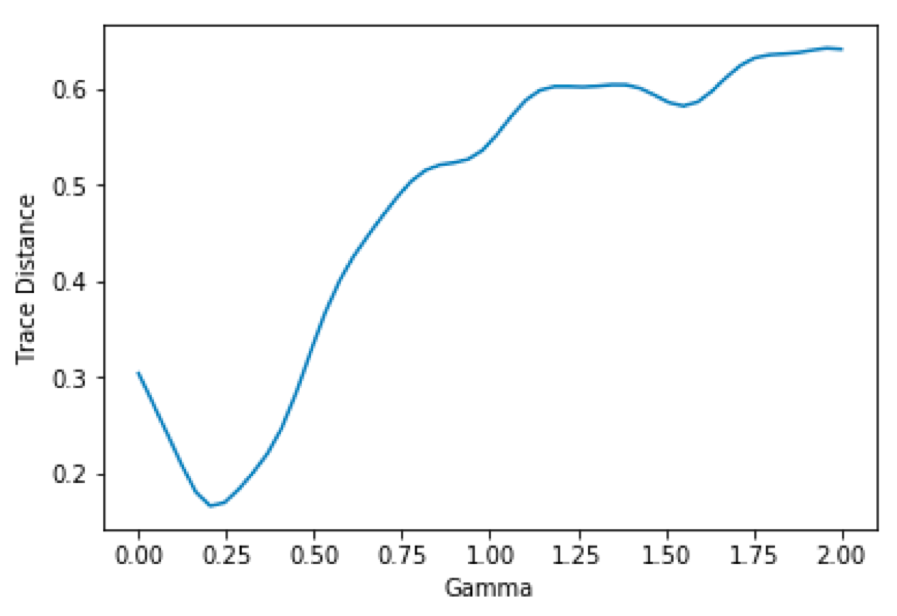
\includegraphics[width=0.5\textwidth]{images/linear_trace_distance}	
\caption{Trace distance as a function of $\gamma$ for a random sample of the UCI Breast Cancer dataset}
\end{figure}

\end{frame}

\subsection{Empirical Evaluation of Tuning by Trace Distance}

\begin{frame}
\begin{itemize}
\item To see that the hypothesized relationship between trace distance and the optimal choice of $\vec{\gamma}$ holds for the roughly linearly separable practical data of the previous section, we performed 20 trials of 200 epochs for linearly spaced $\gamma$ on two sets of 20 random samples of the practical dataset, now requiring that the ratio between $+1$ and $-1$ labelled data points is balanced. 
\item As a result for $\gamma = \{0.0, 0.25, 0.5, 1.0, 1.5, 2.0\}$ we found that the optimal training accuracy was given by $\{ 0.55, 0.55, 0.60, 0.80, 0.85, 0.85 \}$.
\end{itemize}
\end{frame}

\begin{frame}
Now, we consider the Moons dataset over varying $\gamma$

\begin{figure}[H]
\centering
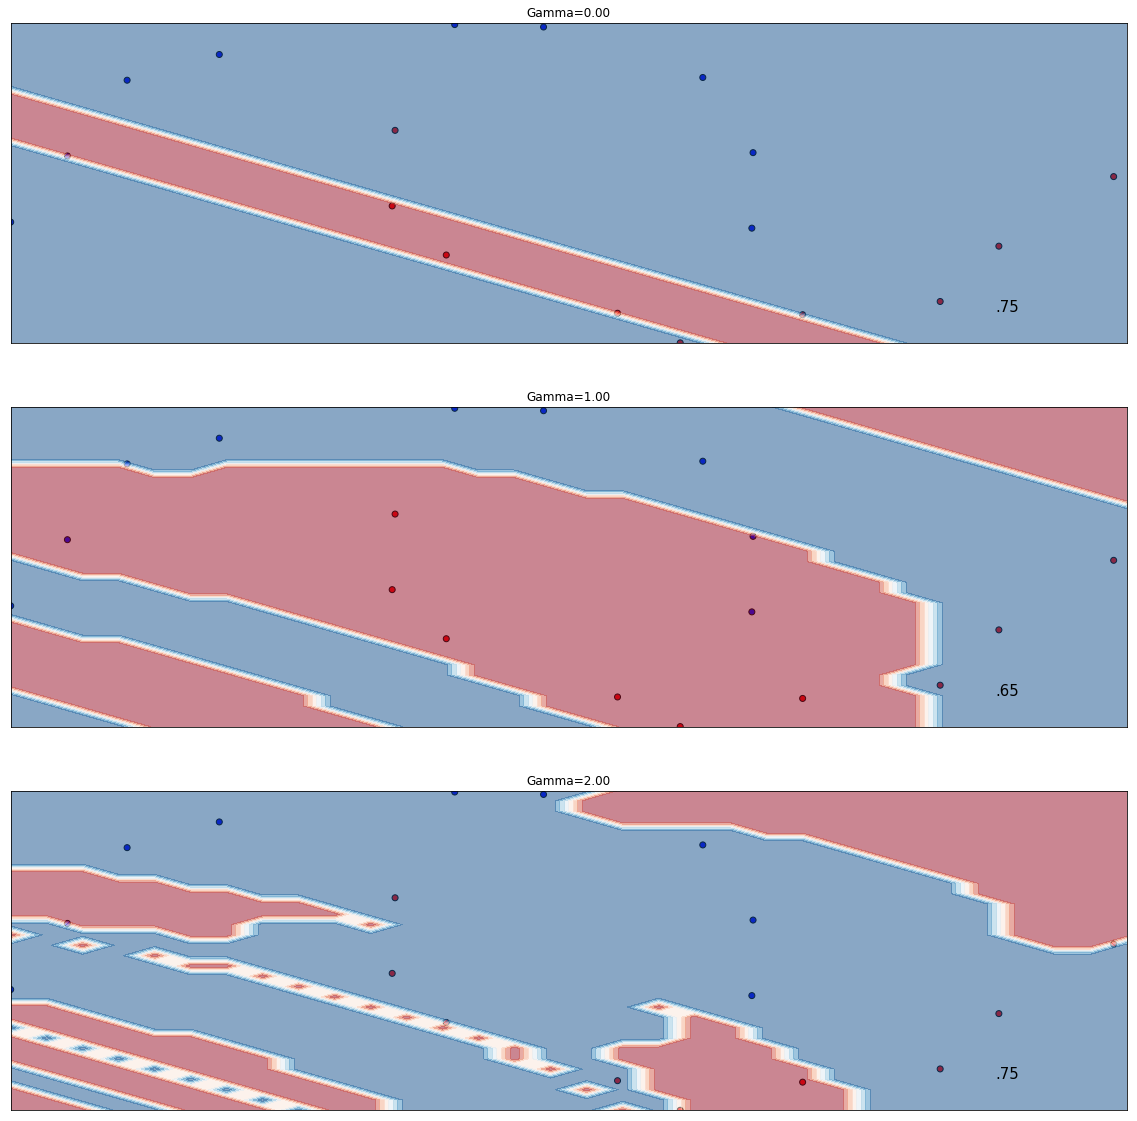
\includegraphics[width=0.5\textwidth]{images/moons_gammas}	
\end{figure}

\end{frame}

\begin{frame}
\begin{figure}[H]
\centering
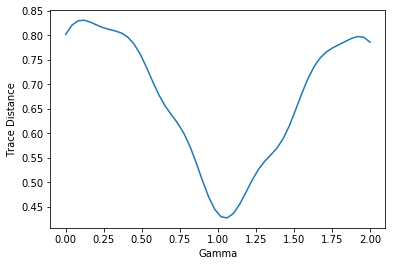
\includegraphics[width=0.5\textwidth]{images/moons_trace_distance}
\caption{The structure of the moons dataset empirically requires a $V$ shaped curve with the trough roughly near $\gamma = 1.0$. Note that such a $\gamma$ is the default value used with no hyper-parameter tuning.}
\end{figure}
\end{frame}

\begin{frame}
So, we expect the classifier to perform relatively poorly for $\gamma=1.0$ and increase towards the extremities. Again, we performed 20 trials of 200 epochs for linearly spaced $\gamma$ on two sets of 20 random samples of the Moons dataset with noise, now requiring that the ratio between $+1$ and $-1$ labelled data points is balanced.
\end{frame}

\begin{frame}

\begin{figure}[H]
\centering
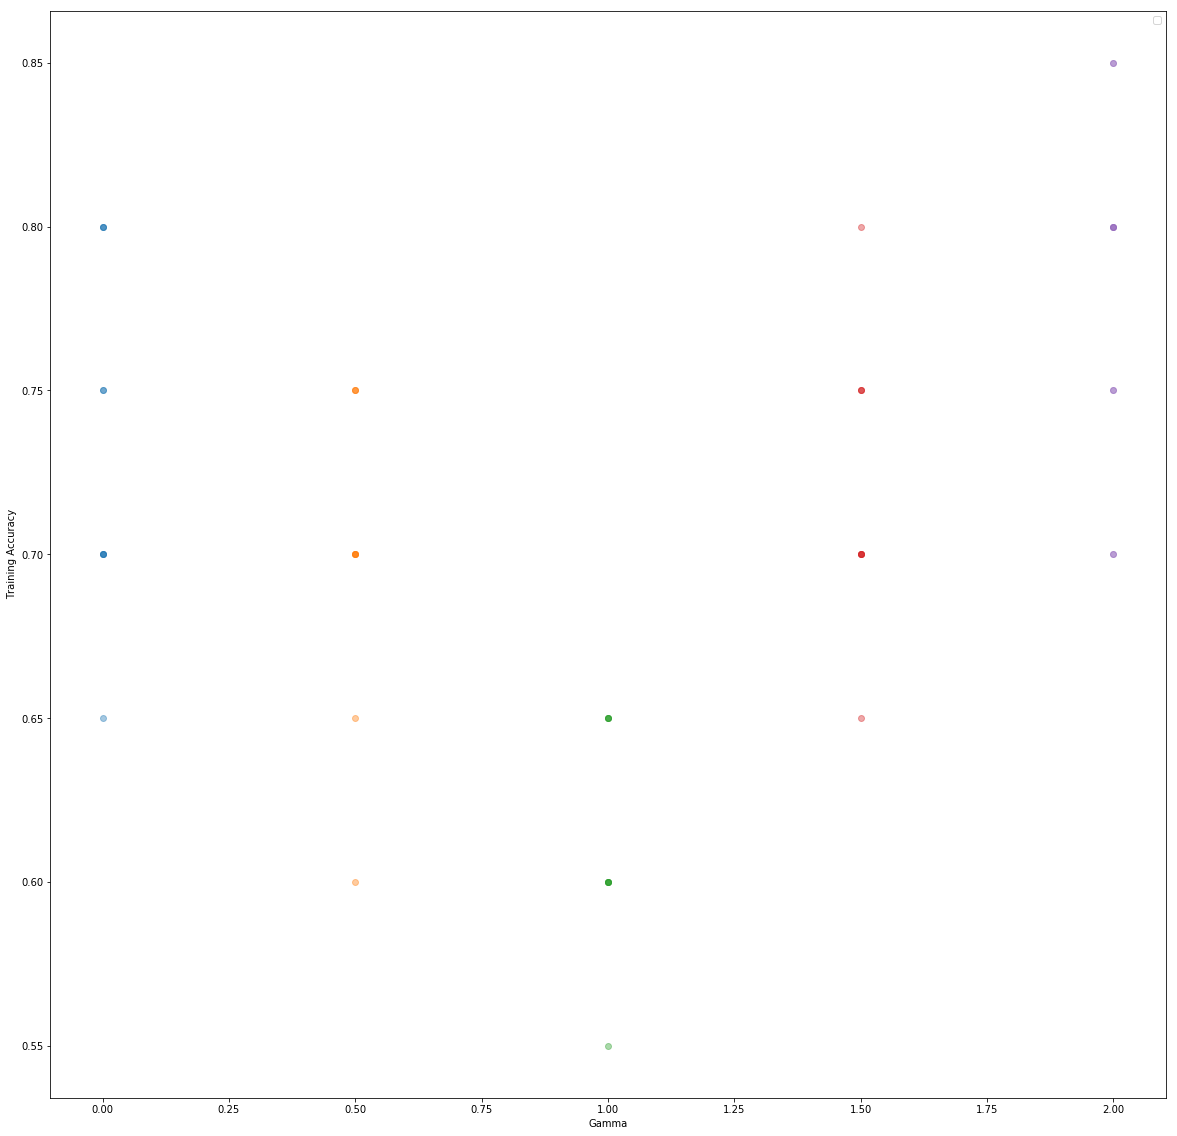
\includegraphics[width=0.7\textwidth]{images/moons_gammas_training}	
\end{figure}
\end{frame}

\begin{frame}
\frametitle{Conclusion}
\begin{itemize}
\item We hope that future works can extend these results and identify additional datasets that have a particular structure for which $\gamma$ ought to be tuned and leave it to these works to verify that trace distance serves a useful purpose to this end.
\item Along these lines, we have open sourced (via GitHub) the code we've used for these simulations
\end{itemize}
\end{frame}

\begin{frame}
\frametitle{Thank you for listening!}
\begin{itemize}
\item I am grateful to the committee for their enthusiasm and willingness to be a part of this defense
\item Questions? fms15@duke.edu
\end{itemize}
\end{frame}


 \end{document}
  
